% !TEX program = pdflatex
\documentclass[9pt]{extarticle}
\usepackage[letterpaper,margin=0.56in,top=0.62in,bottom=0.56in]{geometry}
\usepackage[T1]{fontenc}
\usepackage{lmodern}
\usepackage{graphicx}
\usepackage{amsmath}
\usepackage{booktabs}
\usepackage{tabularx}
\usepackage{array}
\usepackage{caption}
\usepackage{xcolor}
\usepackage{fancyhdr}
\usepackage{titlesec}
\usepackage{enumitem}
\usepackage{hyperref}
\usepackage{microtype}
\usepackage{ragged2e}

\definecolor{navy}{HTML}{193946}
\definecolor{teal}{HTML}{0A7C74}
\definecolor{lightteal}{HTML}{E8F2F1}
\definecolor{amber}{HTML}{D67A35}
\definecolor{lightamber}{HTML}{FFF4E8}
\definecolor{red}{HTML}{B94A48}
\definecolor{lightred}{HTML}{FCEEEE}
\definecolor{slate}{HTML}{526C75}
\definecolor{rulegray}{HTML}{C9D7DA}

\hypersetup{colorlinks=true,urlcolor=teal,linkcolor=teal}
\pagestyle{fancy}
\fancyhf{}
\lhead{\textcolor{slate}{ECG cascade grouped audit}}
\rhead{\textcolor{slate}{Clinician briefing}}
\cfoot{\textcolor{slate}{\thepage\ / 4}}
\renewcommand{\headrulewidth}{0.35pt}
\renewcommand{\footrulewidth}{0pt}
\setlength{\headheight}{12pt}
\setlength{\parindent}{0pt}
\setlength{\parskip}{2.7pt}
\setlist[itemize]{leftmargin=1.15em,itemsep=1.3pt,topsep=2pt}
\setlist[enumerate]{leftmargin=1.3em,itemsep=1.3pt,topsep=2pt}
\titleformat{\section}{\large\bfseries\color{navy}}{}{0pt}{}
\titlespacing*{\section}{0pt}{4pt}{3pt}
\newcolumntype{Y}{>{\RaggedRight\arraybackslash}X}
\newcolumntype{L}[1]{>{\RaggedRight\arraybackslash}p{#1}}
\newcolumntype{C}[1]{>{\centering\arraybackslash}p{#1}}
\newcolumntype{R}[1]{>{\raggedleft\arraybackslash}p{#1}}

\newcommand{\pageheading}[2]{%
  {\fontsize{18}{20}\selectfont\bfseries\color{navy} #1}\par
  {\small\color{slate} #2}\par\vspace{3pt}\color{rulegray}\hrule\color{black}\vspace{5pt}
}
\newcommand{\callout}[3]{%
  \noindent\fcolorbox{#1}{#2}{\parbox{0.965\linewidth}{\small #3}}\par
}
\newcommand{\metric}[2]{\textbf{#1}: #2}

\begin{document}

% -----------------------------------------------------------------------------
% PAGE 1
% -----------------------------------------------------------------------------
\pageheading{Can the feature matrix distinguish the clinical labels?}{A four-page interpretation of 39,664 ECG feature rows using patient/source-grouped out-of-fold testing}

\callout{teal}{lightteal}{\textbf{Bottom line.} The system did \emph{not} predict everything correctly. Across the five selected tasks it made 7,162 target-level errors. Artifact and unusable-signal discrimination were strong internally; abnormal-beat discrimination was moderate; seizure discrimination was weak; and the noise estimate is based on only two independent source patients. None is an external clinical validation.}

\begin{center}
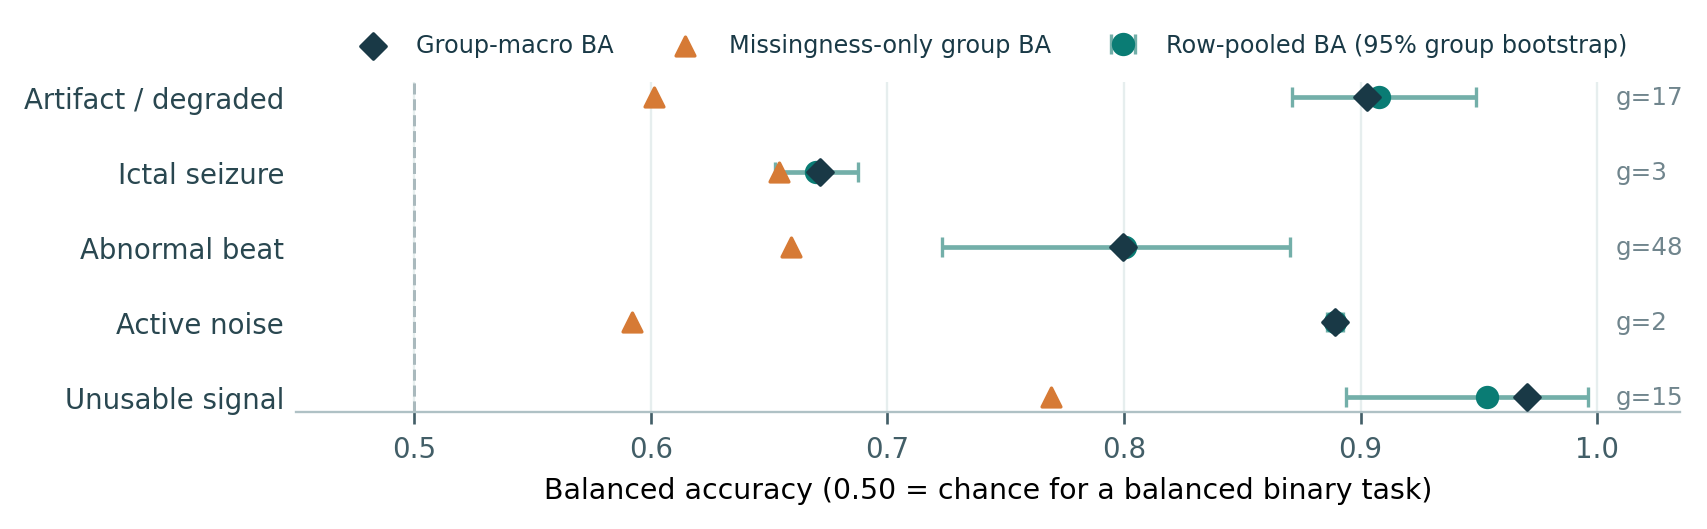
\includegraphics[width=0.985\linewidth]{performance_overview.png}
\end{center}
\vspace{-5pt}

\begin{table}[h!]
\centering
\caption*{Selected out-of-group result for each target. The five target denominators overlap; 46,038 target-level predictions arise from 39,664 unique feature rows.}
\scriptsize
\setlength{\tabcolsep}{3.2pt}
\begin{tabularx}{\linewidth}{@{}L{1.13in}Y C{0.28in} R{0.43in} R{0.43in} R{0.43in} R{0.43in} R{0.48in}@{}}
\toprule
Target & Selected model and feature branch set & $g$ & Sens. & Spec. & PPV & Group BA & Errors \\
\midrule
Artifact / degraded & Logistic regression; B2 morphology + B4 quality & 17 & 87.9\% & 93.7\% & 94.5\% & 90.3\% & 1,077 \\
Ictal seizure & Linear SVM; B1 rhythm/HRV & 3 & 63.0\% & 71.0\% & 19.7\% & 67.1\% & 3,388 \\
Abnormal beat & Histogram boosting; B1+B2+B3 & 48 & 69.9\% & 90.2\% & 64.3\% & 80.0\% & 2,171 \\
Active noise & Linear SVM; B2+B4 & 2 & 82.2\% & 95.7\% & 97.9\% & 88.9\% & 395 \\
Strict unusable & Linear SVM; B2 morphology & 15 & 92.7\% & 98.0\% & 88.0\% & 97.0\% & 131 \\
\bottomrule
\end{tabularx}
\end{table}
\vspace{-5pt}

\section*{How to read the statistics}
\begin{minipage}[t]{0.49\linewidth}\small
\metric{Sensitivity}{of all true positive episodes/rows, the fraction detected: $TP/(TP+FN)$. A low value means clinically relevant misses.}

\metric{Specificity}{of all true negatives, the fraction correctly rejected: $TN/(TN+FP)$. A low value means excess alarms.}

\metric{PPV (precision)}{of all positive alerts, the fraction truly positive: $TP/(TP+FP)$. It depends strongly on prevalence.}
\end{minipage}\hfill
\begin{minipage}[t]{0.49\linewidth}\small
\metric{Balanced accuracy (BA)}{$\tfrac12$(sensitivity + specificity). It gives equal weight to both classes and is more informative than ordinary accuracy in an imbalanced dataset.}

\metric{Group-macro BA}{sensitivity and specificity are first calculated per independent lineage, then averaged. A long recording cannot dominate many shorter patients.}

\metric{95\% group bootstrap}{1,000 resamples of whole lineages, not correlated beats. The plotted interval is for row-pooled BA; the diamond is group-macro BA.}
\end{minipage}

\vfill
{\scriptsize\color{slate}\textbf{Audit design:} 5 targets $\times$ 5 classifier families $\times$ all 15 non-empty branch combinations = 375 experiments. Every displayed prediction came from a fold that excluded its complete lineage group; preprocessing was fitted inside the training fold.}

\newpage

% -----------------------------------------------------------------------------
% PAGE 2
% -----------------------------------------------------------------------------
\pageheading{Group clusters: where performance is stable or fragile}{Each point is one independent patient/source lineage with both positive and negative examples; bars show the interquartile range and median}

\begin{center}
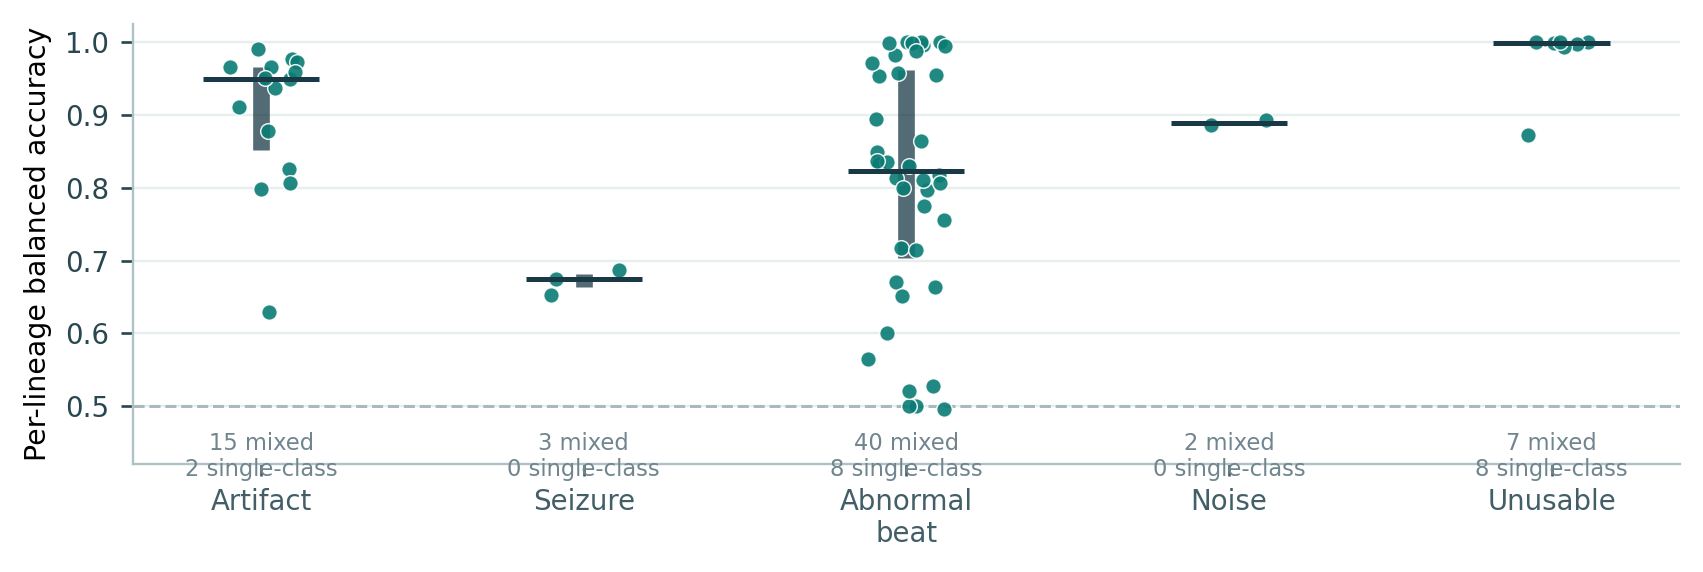
\includegraphics[width=0.99\linewidth]{group_variability.png}
\end{center}
\vspace{-6pt}

\begin{table}[h!]
\centering
\caption*{Distribution across independent lineages. ``Single class'' means that BA is mathematically undefined because the group contains only positives or only negatives.}
\scriptsize
\setlength{\tabcolsep}{4pt}
\begin{tabularx}{0.94\linewidth}{@{}Y C{0.42in} C{0.48in} C{0.68in} C{0.64in} C{0.48in} C{0.48in}@{}}
\toprule
Target & All $g$ & Mixed $g$ & Median BA & IQR & BA $<$.60 & BA $\geq$.80 \\
\midrule
Artifact & 17 & 15 & 95.0\% & 85.2--96.6\% & 0 & 13 \\
Seizure & 3 & 3 & 67.4\% & 66.3--68.1\% & 0 & 0 \\
Abnormal beat & 48 & 40 & 82.3\% & 70.3--96.1\% & 6 & 24 \\
Active noise & 2 & 2 & 88.9\% & 88.7--89.1\% & 0 & 2 \\
Strict unusable & 15 & 7 & 99.9\% & 99.5--100\% & 0 & 7 \\
\bottomrule
\end{tabularx}
\end{table}
\vspace{-5pt}

\section*{Three evidence clusters}
\begin{enumerate}
\item \textbf{Broader but heterogeneous internal evidence - abnormal beats.} Forty-eight independent lineages are represented, yet six of the 40 mixed-class lineages score below 60\% BA. The aggregate 80.0\% group BA therefore hides clinically important record-to-record variation.
\item \textbf{Limited internal evidence - artifact and unusable signal.} Artifact covers 17 groups and is usually stable, but the worst mixed group is 63.0\% BA. Unusable signal is excellent in seven mixed groups, while eight other groups contain only one class and cannot test both sensitivity and specificity.
\item \textbf{Critical sample-size limitation - seizure and active noise.} Seizure has only three patients/source groups and no group reaches 80\% BA. Active noise appears strong but comes entirely from MIT-BIH source patients 118 and 119. Two similar patients cannot establish generalization.
\end{enumerate}

\callout{amber}{lightamber}{\textbf{Why the seizure number is not reassuring.} The seizure classifier finds 728 of 1,156 ictal rows (63.0\% sensitivity) but produces 2,960 false-positive rows. PPV is only 19.7\%: about four of five positive alerts are false in this selected corpus. A feature-missingness-only model reaches 65.4\% group BA, close to the selected model's 67.1\%.}

\section*{What the four feature branches mean}
\small
\textbf{B1 rhythm/physiology} (RR, heart-rate variability, PRSA/BPRSA); \textbf{B2 morphology} (template similarity and P-QRS-T shape); \textbf{B3 conduction/repolarization} (PR, QT, JT and related intervals); \textbf{B4 quality} (flatness, spectral ratios, detector agreement and template support). The audit tested every non-empty combination, but the group clusters above - not the winning branch label alone - determine how much confidence is warranted.

\vfill
{\scriptsize\color{slate}\textbf{Negative controls:} mean BA after 20 training-label permutations was 48.5\% abnormal, 48.2\% artifact, 54.2\% noise, 50.3\% seizure and 49.1\% unusable. Near-chance permutations are necessary evidence against direct leakage, but they do not prove external validity.}

\newpage

% -----------------------------------------------------------------------------
% PAGE 3
% -----------------------------------------------------------------------------
\pageheading{Mixed clinical contexts: what can and cannot be measured}{Joint labels exist for noise, artifact and beat type in NSTDB; seizure-plus-noise/artifact/beat combinations are not annotated}

\begin{center}
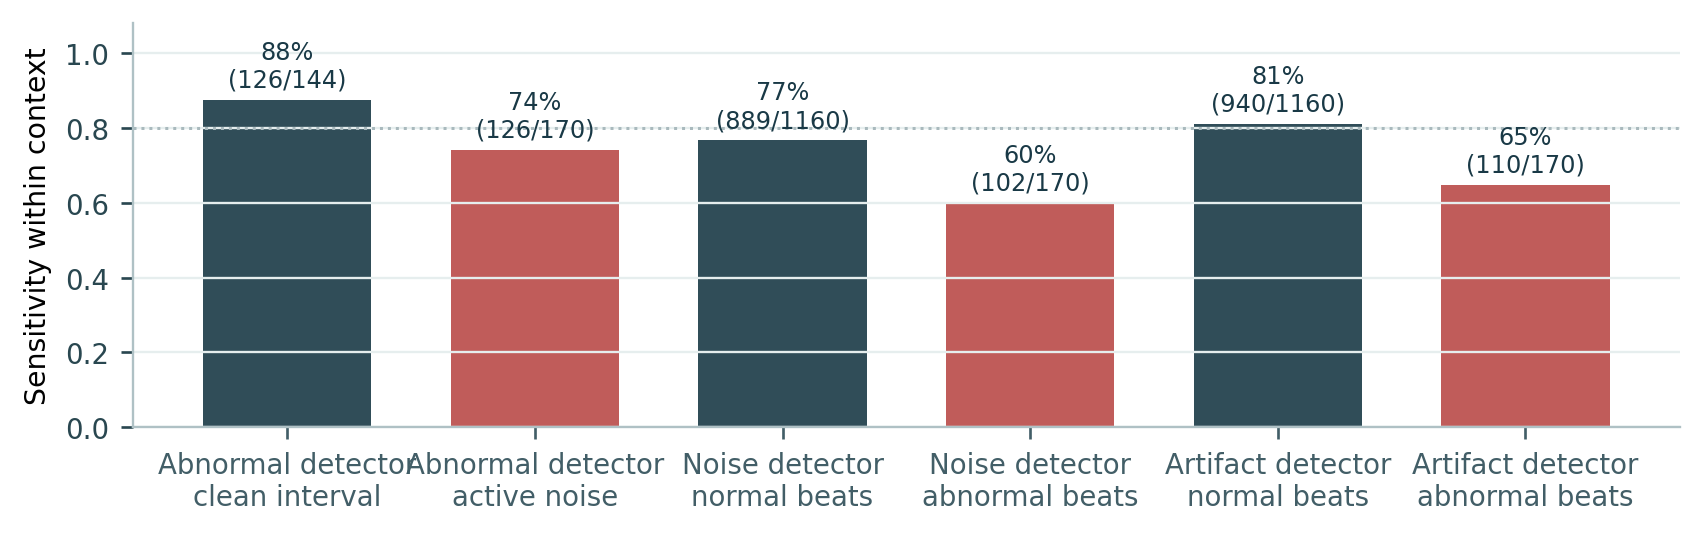
\includegraphics[width=0.99\linewidth]{mixed_context.png}
\end{center}
\vspace{-5pt}

\callout{red}{lightred}{\textbf{Clinically important interaction.} In NSTDB, abnormal-beat sensitivity falls from 88\% in clean intervals (126/144) to 74\% during active noise (126/170). Among truly noisy rows, noise sensitivity falls from 77\% on normal beats (889/1,160) to 60\% on abnormal beats (102/170). Artifact sensitivity similarly falls from 81\% to 65\%. Abnormal morphology and noise can therefore mask one another.}

\section*{Observed joint classes in NSTDB}
\begin{minipage}[t]{0.42\linewidth}
\centering
\scriptsize
\begin{tabular}{@{}lrrr@{}}
\toprule
Context & Normal beat & Abnormal beat & Total \\
\midrule
Clean interval & 684 & 144 & 828 \\
Active noise/artifact & 1,160 & 170 & 1,330 \\
\midrule
Total & 1,844 & 314 & 2,158 \\
\bottomrule
\end{tabular}
\end{minipage}\hfill
\begin{minipage}[t]{0.55\linewidth}\small
These 2,158 rows have both an expert-matched beat class and the official noise schedule. The remaining 689 NSTDB rows retain noise/artifact truth but have no attached abnormal-beat target. Unknown labels were excluded, not changed to class 0.

The artifact and noise labels are identical in NSTDB by design: official inactive interval = 0 and active interval = 1. They are \emph{different models}, however, because the artifact target is also trained on BUT-QDB quality labels.
\end{minipage}

\section*{Quality-severity classes in BUT-QDB}
\small
The composite artifact analysis contains 4,221 class-1 usable rows, 3,593 class-2 degraded rows and 656 class-3 unusable rows. The artifact model correctly rejects 96.1\% of class 1, detects 87.8\% of class 2 and detects 94.2\% of class 3. The stricter unusable task compares class 1 versus class 3 only; class 2 is deliberately excluded because ``degraded'' is not the same clinical endpoint as ``unusable.'' The official three-class definitions and 15-subject structure are documented by \href{https://physionet.org/content/butqdb/1.0.0/}{PhysioNet BUT-QDB}.

\section*{Why seizure plus noise/abnormal/artifact is marked ``not evaluable''}
\begin{tabularx}{\linewidth}{@{}L{1.45in}Y L{1.10in}@{}}
\toprule
Requested combination & What the present data contain & Defensible conclusion \\
\midrule
Seizure + active noise & Seizure intervals in CHB-MIT/Siena; no synchronized NSTDB noise truth & Not evaluable \\
Seizure + abnormal beat & Seizure intervals; no expert AAMI beat labels in the seizure rows & Not evaluable \\
Seizure + artifact/unusable & Seizure intervals; no BUT-QDB quality consensus in those recordings & Not evaluable \\
Noise + abnormal beat & Both labels coexist in 2,158 NSTDB rows & Evaluated above \\
Artifact + unusable & Both labels coexist in pure BUT-QDB class 1/3 windows & Severity analysis \\
\bottomrule
\end{tabularx}

\callout{teal}{lightteal}{\textbf{Do not read ``not evaluable'' as zero.} It means the necessary joint ground truth was never recorded in the same observations. Training a model to invent those missing labels would create an apparently complete but scientifically invalid matrix.}

\vfill
{\scriptsize\color{slate}NSTDB's stress recordings are constructed from only MIT-BIH 118 and 119 and use alternating noise intervals; see \href{https://physionet.org/content/nstdb/1.0.0/}{PhysioNet NSTDB}. This explains both the useful mixed-context analysis and the severe two-patient limitation.}

\newpage

% -----------------------------------------------------------------------------
% PAGE 4
% -----------------------------------------------------------------------------
\pageheading{Case studies: concrete successes, misses and false alarms}{Record-level results make the aggregate percentages clinically interpretable}

\begin{table}[h!]
\footnotesize
\setlength{\tabcolsep}{3pt}
\begin{tabularx}{\linewidth}{@{}L{0.82in}L{0.78in}L{1.58in}Y L{1.58in}@{}}
\toprule
Task & Record / group & Exact result & What failed & Clinical reading \\
\midrule
Seizure & PN06\_5 / PN06 & 1,079 rows: TP 22, FN 49, TN 681, FP 327; BA 49.3\%; PPV 6.3\% & Most ictal rows were missed and many non-ictal rows alerted. & A near-chance record despite the aggregate 67.1\% group BA; unsuitable for alarm use. \\
Artifact & NSTDB 118e24 / 118 & 233 rows: TP 41, FN 116, TN 72, FP 4; BA 60.4\% & Sensitivity only 26.1\%; the model was conservative. & A clean-looking negative output cannot reliably exclude artifact in this record. \\
Active noise & NSTDB 118e24 / 118 & 233 rows: TP 66, FN 91, TN 65, FP 11; BA 63.8\% & Sensitivity 42.0\% despite 85.5\% specificity. & The overall 88.9\% hides a clinically weak record/window selection. \\
Abnormal beat & MIT-BIH 207 / 207 & 103 abnormal rows: TP 36, FN 67; sensitivity 35.0\% & Two thirds of abnormal anchors were classified normal. Specificity is undefined because this selected window has no negatives. & Demonstrates why single-record accuracy and pooled specificity must not be substituted for sensitivity. \\
Strict unusable & BUT 111001 / 111 & 289 rows: TP 137, FN 47, TN 105, FP 0; BA 87.2\% & No false unusable alarms, but 25.5\% of unusable rows were missed. & Strong aggregate behavior still permits a clinically meaningful false-reassurance mode. \\
\bottomrule
\end{tabularx}
\end{table}

\section*{Strengths demonstrated by the audit}
\begin{itemize}
\item The raw inventory byte-read and SHA-256-hashed 4,856 files (8.15 GB) with zero read errors. Six isolated reconstructions reproduced all 39,664 row IDs, all 52 feature values and all 56 semantic label fields with zero differences.
\item Ten separate label-semantic checks found zero mismatches. Exact duplicate feature vectors never crossed lineage groups. All 375 experiment cells retained complete out-of-fold predictions.
\item Artifact was strong in most mixed groups (median BA 95.0\%; 13/15 groups at least 80\%). Abnormal-beat performance was useful in many lineages (24/40 at least 80\%) but clearly heterogeneous.
\end{itemize}

\section*{Defects and boundaries that remain}
\begin{itemize}
\item \textbf{No external cohort.} The displayed winner was selected on the same cross-validation matrix. It is an inspection winner, not an unbiased final-test estimate.
\item \textbf{Curated rather than full-waveform evidence.} The matrix contains 336 label-rich segments. A separate plan covers 557.81 raw signal-hours and 11,337 windows, but unlabelled windows were not fabricated as negatives.
\item \textbf{Beat-classification boundary.} Abnormal truth is attached only when a pipeline beat anchor lies within 75 ms of an expert beat. Expert beats missed by the detector produce no classifier row, so this is not end-to-end detection sensitivity.
\item \textbf{Shortcuts remain possible.} Missingness-only group BA is 65.4\% for seizure and 76.9\% for unusable signal. Source acquisition and feature availability can carry label information.
\end{itemize}

\callout{amber}{lightamber}{\textbf{Clinical interpretation.} These results justify continued engineering evaluation of artifact, morphology and abnormal-beat features. They do not justify diagnosis, seizure alarms or automated signal rejection. The next valid test requires patient-unique external data with joint seizure, beat-type and signal-quality annotation, plus an end-to-end accounting of missed detector beats.}

\vfill
{\scriptsize\color{slate}\textbf{Reporting basis.} Grouped validation and transparent denominators follow the intent of \href{https://www.bmj.com/content/385/bmj-2023-078378}{TRIPOD+AI}. Dataset-only and missingness-only controls address shortcut risks described in \href{https://www.nature.com/articles/s41746-024-01118-4}{medical-AI shortcut-learning research}. Generated from audit version 2.0.0, matrix SHA-256 \texttt{2e7751f2894343fa367c790f41af2e0f...}.}

\end{document}
